\documentclass[pdftex,12pt,letterpaper]{extarticle}

%%% Set these variables appropriately
%%%
%% Note:  Authors is hardcoded below, this line only used for the PDF info
\newcommand{\AUTHORS}{Submitted by: Conglong Li}
\newcommand{\TITLE}{}
\newcommand{\KEYWORDS}{Put your keywords here}
\newcommand{\CONFERENCE}{Somewhere}
\newcommand{\PAGENUMBERS}{yes}       % "yes" or "no"
\newcommand{\COLOR}{yes}
\newcommand{\showComments}{yes}
\newcommand{\comment}[1]{}
\newcommand{\onlyAbstract}{no}

%%%%%%%%%%%%%%%%%%%%%%%%%%%%%%%%%%%%%%%%%%%%%%%%%%%%%%%%%%%%%%%%%%%%%

%%%
%%%  Page Setup
%%%
\special{papersize=8.5in,11in}
\setlength{\pdfpagewidth}{8.5in}
\setlength{\pdfpageheight}{11in}

\usepackage{ifthen}
\ifthenelse{\equal{\PAGENUMBERS}{yes}}{%
\usepackage[nohead,
            left=1in,right=1in,top=1in,
            footskip=0.5in,bottom=1in,     % Room for page numbers
            columnsep=0.25in
            ]{geometry}
}{%
\usepackage[noheadfoot,left=0.75in,right=0.85in,top=0.75in,
            footskip=0.5in,bottom=1in,
            columnsep=0.25in
	    ]{geometry}
}

%%% Alter some LaTeX defaults for better treatment of figures:
%%% See p.105 of "TeX Unbound" for suggested values.
%%% See pp. 199-200 of Lamport's "LaTeX" book for details.
%%%   General parameters, for ALL pages:
\renewcommand{\topfraction}{0.9}	% max fraction of floats at top
\renewcommand{\bottomfraction}{0.8}	% max fraction of floats at bottom
%%%   Parameters for TEXT pages (not float pages):
\setcounter{topnumber}{2}
\setcounter{bottomnumber}{2}
\setcounter{totalnumber}{4}     % 2 may work better
\setcounter{dbltopnumber}{2}    % for 2-column pages
\renewcommand{\dbltopfraction}{0.99}	% fit big float above 2-col. text
\renewcommand{\textfraction}{0.01}	% allow minimal text w. figs
%%%   Parameters for FLOAT pages (not text pages):
\renewcommand{\floatpagefraction}{0.99}	% require fuller float pages
%%% N.B.: floatpagefraction MUST be less than topfraction !!
\renewcommand{\dblfloatpagefraction}{0.7}	% require fuller float pages


%%%
%%%  Captions
%%%
\usepackage[font=bf]{caption}
%%  Space between figure and caption (assuming caption
%%  is below figure)
%\usepackage[font=bf,aboveskip=0pt]{caption} % SPACE
%%  Space between caption and body text of document
\addtolength{\textfloatsep}{-7pt} % SPACE

%%%
%%%  Section headings
%%%
%\usepackage{titlesec}
%\titlespacing{\paragraph}{0pt}{*1}{*1}      % SPACE
\usepackage[compact]{titlesec}              % SPACE
%\titleformat{\section}%                     % IEEE/ACM: caps + period
%  {\bf\large\uppercase}{\thesection.\quad}{0pt}{}

%%%
%%%  Lists
%%%
\usepackage{enumitem}
\setlist{itemsep=0pt,parsep=0pt}             % more compact lists

%%%
%%%  Header / Footer
%%%
\usepackage{fancyhdr}
\renewcommand{\headrulewidth}{0pt}

\ifthenelse{\equal{\PAGENUMBERS}{yes}}{%
  \pagestyle{plain}
}{%
  \pagestyle{empty}
}

%%%
%%%  Bibliography
%%%
\usepackage[numbers]{natbib}

%%%
%%%  Footnotes / Endnotes
%%%
\interfootnotelinepenalty=10000  % Split footnotes are annoying

% If you want endnodes, uncomment:
%\usepackage{endnotes}
%\usepackage{drafthead}
%\let\footnote=\endnote

%%%
%%%  Tables
%%%
\usepackage{booktabs}
\usepackage{color}
\usepackage{colortbl}
\usepackage{float}                           % Must appear before hyperref to
                                             % avoid weird PDF compile issues

%%%
%%%  Fonts
%%%
\usepackage{mathptmx}                        % Times/Times-like math symbols
\usepackage{courier}
\usepackage[scaled=0.92]{helvet}


%%%
%%% Script letters
%%%
\usepackage[mathscr]{euscript}
\usepackage[T1]{fontenc}
%%%
%%% Code
%%%
\usepackage{listings}
\usepackage{inconsolata}
\definecolor{dkgreen}{rgb}{0,0.6,0}
\definecolor{gray}{rgb}{0.5,0.5,0.5}
\definecolor{mauve}{rgb}{0.58,0,0.82}

\lstset{
	language=C,
	moredelim=**[is][\color{magenta}]{@}{@},
	moredelim=**[is][\color{dkgreen}]{`}{`},
    commentstyle=\color{dkgreen},
  	keywordstyle=\color{blue},
    stringstyle=\color{mauve},
  	numberstyle=\footnotesize\ttfamily\color{gray},
  	basicstyle={\footnotesize\ttfamily},
    breakatwhitespace=false,         
    breaklines=true,                 
    captionpos=b,                    
    keepspaces=true,                 
    numbers=left,                    
    numbersep=5pt,                  
    showspaces=false,                
    showstringspaces=false,
    showtabs=false,                  
    tabsize=2,
	xleftmargin=2em,						% Line numbers inside frame
	framexleftmargin=1.5em,					% Line numbers inside frame
}

% Add extra keywords for code listing here
\lstset{emph = {value\_t, entry\_t, key\_t}, emphstyle = {\color{blue}},%
		emph = {g\_label\_0, g\_label\_1, g\_label\_2, g\_end}, emphstyle = {\color{magenta}}
}

\renewcommand{\lstlistingname}{Algorithm}

%%%
%%%  PDF setup
%%%
\ifthenelse{\equal{\COLOR}{yes}}{%
  \usepackage[colorlinks]{hyperref}%         % for online version
}{%
  \usepackage[pdfborder={0 0 0}]{hyperref}%  % for paper (B&W) version
}
\usepackage{url}

\hypersetup{%
pdfauthor = {\AUTHORS},
pdftitle = {\TITLE},
pdfsubject = {\CONFERENCE},
pdfkeywords = {\KEYWORDS},
bookmarksopen = {true}
}

%%
%% Figure placeholder macros
%%
\usepackage[font={small,it}]{subfig}
\definecolor{placeholderbg}{rgb}{0.85,0.85,0.85}
\newcommand{\placeholder}[1]{%
\fcolorbox{black}{placeholderbg}{\parbox[top][1.5in][c]{0.95\columnwidth}{#1}}}


%%%
%%%  Misc
%%%
\usepackage[pdftex]{graphicx}
\usepackage{soul}

%\setlength{\parindent}{0pt}
%\setlength{\parskip}{\baselineskip}

%\clubpenalty=10000  % Don't allow orphans
%\widowpenalty=10000 % Don't allow widows

%%%
%%%  To appear/appeared in text on title page
%%%
\usepackage[absolute]{textpos}
\newcommand{\ToAppear}{%
\begin{textblock*}{\textwidth}(0.95in,0.4in)
\begin{flushright}
    %\noindent{\fbox{\textsf{Under submission---please do not redistribute.}}}
    %  --OR--
    \noindent{\small To appear in \textit{Proceedings of the XYZ}\\
    \noindent{\small \textit{Conference (XYZ'08)}, City, State, Month 2008}}
    %  --OR--
    %\noindent{\small In \textit{Proceedings of the XYZ}\\
    %\noindent{\small \textit{Conference (XYZ'08)}, City, State, Month 2008}}
\end{flushright}
\end{textblock*}
}

%%%
%%%  Sample ACM Copyright Block
%%%
\newfloat{acmcr}{b}{acmcr}
\newcommand{\AcmCopyright}{%
\begin{acmcr}
\parbox[b]{20pc}{%
\footnotesize
Permission to make digital or hard copies of all or part of this work
for personal or classroom use is granted without fee provided that
copies are not made or distributed for profit or commercial advantage
and that copies bear this notice and the full citation on the first
page.  To copy otherwise, to republish, to post on servers or to
redistribute to lists, requires prior specific permission and/or a fee.

{\em Conference}, Month Date--Date, Year, Location\\
Copyright 200X ACM X-XXXXX-XX-X/XX/XX ...\$5.00}
\end{acmcr}}

%%%
%%%  Comments
%%%
%\newcommand{\note}[2]{
%    \ifthenelse{\equal{\showComments}{yes}}{\textcolor{#1}{#2}}{}
%}
\newcommand{\note}[2]{
  \ifthenelse{\equal{\showComments}{yes}}{\textcolor{#1}{\sf\small\fontfamily{phv}\fontseries{mc}\selectfont#2}}{}
}

% Change these to your own initials as you like...
\newcommand{\dga}[1]{\note{blue}{DGA: #1}}
\newcommand{\mk}[1]{\note{red}{MK: #1}}
\newcommand{\dz}[1]{\note{green}{DZ: #1}}
\newcommand{\ak}[1]{\textcolor{red}{#1}}

\date{}
\title{\textbf{\TITLE 15-712 Project Report\\ Introduce Indirection Scheduling \\to Datacenter Hybrid Switch}}
\author{{\large Conglong Li, Anbang Zhao}\\
{\em $\left\{conglonl, anbangz\right\}@andrew.cmu.edu$}}


% This needs to be the last thing before \begin{document}
\usepackage{microtype}  % SPACE

%%%%%%%%%%%%%%%%%%%%  START DOCUMENT  %%%%%%%%%%%%%%%%%%%%%%%%
\begin{document}

\maketitle

%\AcmCopyright
%\ToAppear

\section{Introduction}

Traditionally, circuit switching and packet switching have been
considered as alternative design choices, each with their own advantages
and disadvantages. Packet switches are efficient at multiplexing traffic
across a large number of ports, while circuit switches can often service
higher line rates in a more cost-effective manner, especially when
combined with optical links. However, as optical circuit switching
technology advances, the reconfiguration time (i.e., the amount of time
it takes to alter the input-to-output mapping) is swiftly decreasing,
thus increasingly blurring the division between the packet and circuit
regimes.

One key domain in which these design tradeoffs are being revisited today
is datacenter switching. The datacenter environment, aggregating
tremendous amounts of compute and storage capacity, has driven demand
for ever increasing port counts and line speeds. However, supporting
these demands with existing packet switching technology is becoming
increasingly expensive—in cost, heat and power. Moreover, studies have
shown that the traffic demand inside a datacenter (both within and
across racks) is frequently highly nonuniform, with a large fraction of
the traffic at each switch port destined for a small number of output
ports~\cite{Kandula:2009-2}.

Based on these observations, researchers had proposed hybrid datacenter
network architectures that offer higher throughputs at lower cost by
combining switching technologies. In particular, recent proposals
suggest employing highspeed optical~\cite{Chen:2012, Farrington:2010,
Wang:2010} or wireless~\cite{Halperin:2011, Kandula:2009, Zhou:2012}
networks configured to service the heavy flows, while passing the
remainder of the traffic through a traditional, relatively
underprovisioned packet-switched network. 

As technology trends usher in dramatically faster reconfiguration times,
the distinction between packet and circuit is blurred, and ever smaller
flows can take advantage of a hybrid fabric. This trend will soon allow
servicing the bulk of the traffic through a rapidly reconfigurable
optical switch~\cite{Porter:2013}, leaving a relatively minor portion to
be serviced by the packet network~\cite{Liu:2014}. While the potential
cost savings that hybrid technologies could realize is large, the design
space for scheduling resources in the hybrid regime is not yet well
understood. 

Many of the classical approaches to scheduling for switches with
non-trivial reconfiguration delays divide the offered demand into two
parts: an initial, heavy-weight component that is served by O(N) highly
utilized configurations with significant durations, and a second,
residual component that is serviced by a similar number of short,
under-utilized schedules. Recent Solstice scheduling
algorithm~\cite{Liu:2014} exploits the skewed nature of datacenter
traffic patterns to create a small number of configurations with long
durations that minimize the penalty for reconfiguration and leaves only
a small amount of residual demand to be serviced by a low-speed (and
lowcost) unconstrained packet switch.

To ensure high overall circuit utilization, each circuit configuration
must be maintained for a relatively long period with respect to the
reconfiguration delay. This leads to two issues for the scheduling
algorithm: Since the demand is skewed, the demands served by a single
configuration could have a large variation. Thus a portion of the links
in optical switch could be under-utilized. Since the configuration time
is still non-trivial, it is still hard to schedule small traffic demands
efficiently on optical switch. Scheduling algorithms are forced to serve
these small demands by packet switch, which is slower and less
cost-effective.

To increase the utilization rate of the optical switches and to reduce the
number of configurations, we propose an indirection scheduling technique: instead
of scheduling each demand with unique direct path, we could leverage existing
paths to serve some demands indirectly. Using this technique, scheduling algorithm
could reduce the skewness of the demands and reduce the number of configurations.

The evaluation of the indirection technique has two objectives. The
first is to find out the optimal possible benefit of indirection. We
achieved this goal by formulating the scheduling problem into an integer
linear programming (ILP) problem. Using $Gurobi$ ILP
solver~\cite{Gurobi} to compare the optimal solution with and without
indirection, we show that using indirection could reduce the number of
configurations and the total transmission time.

The second objective is to find out the practical benefit of indirection.
We achieved this goal by simulations of hybrid switch scheduling. We implemented
two simple indirection heuristics and applied them to the Solstice algorithm.
Comparing the simulations of Solstice algorithm with and without
indirection heuristics, results show that even simple indirection
heuristics could provide improvements above direct path algorithm.
Although our indirection heuristics didn't approach similar amount
of improvement as in the ILP formulation results, we argue that better
improvement is possible with clever indirection heuristics embedded with
the scheduling algorithm.

The rest of this report is organized as follows. Section~\ref{sec:ilp}
described the ILP formulation and the solver results.
Section~\ref{sec:simres} describes the preliminary indirection
heuristics and the simulation results. Finally, we summarize this
project in Section~\ref{sec:conclusion}.

\section{ILP Formulation of the Scheduling Problem}
\label{sec:ilp}

\subsection{Problem Formulation}
Integer linear programming is a mathematical optimization method. An
integer linear program is expressed with a minimization/maximization
objective function, constraints of the variables, and bounds of the
variables. For our scheduling problem, the objective function is clearly
the minimization of the total transmission time, but the constraints are
complicated. In the remaining of this section, we will describe the
constraints implemented in the program.

\paragraph{Input Demand Matrix}
To define the input of each integer linear program, we defined the demands
needs to be served as a N by N matrix, where N is the number of ports in the
network. Entry (a, b) in the input demand matrix denotes the amount of demand
to be transfered from port a to port b. Each (a, a) entry has zero demand.
Then we ask the program to solve the scheduling problem so that each demand in
the input demand matrix must be served by either optical or packet switch.

\paragraph{Optical Switch Constraints}
To define the optical switch, we need to implement the concept of configurations.
Each configuration is a matrix that denotes the demands served by this
configuration. Since the input-output mapping is fixed in a single configuration,
each row and each column can only have no more than one non-zero entry.
For each new configuration scheduled, an additional reconfiguration time
is added to the total transmission time. 

\paragraph{Packet Switch Constraints}
Packet switch constraints are different. Packet switch doesn't have the concept
of configurations. It could schedule arbitrary amount of demands on each link
without any reconfiguration time. However, packet switch has less capacity than
optical switch. Thus it could only schedule a smaller fraction of demands within
the same time duration. In our constraints, we configure the packet switch to
have $1/10$ capacity of the optical switch. 

\paragraph{Indirection Technique Constraints}  
To define the indirection technique, we defined each possible indirection decision
in the program. If a decision is made that certain amount of demand from port a
to port b will be indirectly served by paths a -> c and c -> b, the input demand matrix
will reduce the demand in entry (a, b) and increase the demands in entries (a, c)
and (c, b). 

\subsection{ILP Solving Results}

\begin{table}
\centering
{
\begin{tabular}{l|r|r|r|r}
\toprule
\bf Optimal Total Time & \bf Random $\delta$ = 5 & \bf Random $\delta$ = 10 & \bf Random $\delta$ = 20 & \bf Skewed $\delta$ = 10 \\
\midrule
Orig & 100\% & 100\% & 100\% & 100\% \\
Indi & 93.93\% & 90.65\% & 83.8\% & 97.9\% \\
\bottomrule
\end{tabular}
}
\caption{Normalized average optimal solution achieved by direct path scheduling (Orig) and indirection technique (Indi), $\delta$ is the reconfiguration time.}
\label{tab:ilp}
\end{table}

\begin{figure}
	\centering
	\begin{minipage}{3in}%
		\includegraphics[width=3in]{figures/avg-5-rand}
		\caption{Optimal solution count for different number of configurations with random demand}
		\label{fig:5rand}
	\end{minipage}%
	\qquad
	\begin{minipage}{3in}%
		\includegraphics[width=3in]{figures/avg-5-skew}
		\caption{Optimal solution count for different number of configurations with skewed demand}
		\label{fig:5skew}
	\end{minipage}%
\end{figure}

We used the Gurobi ILP solver to solve the optimal solutions of our
integer linear programs. Since integer linear solving is NP-hard, we
choose to solve 5 by 5 input demand matrix. This is a small input
compared to the matrix used in the simulator. But it is big enough to
show the potential benefit of the indirection technique.

We used two different kinds of workload. The first is random workload
where each entry has a demand randomly chosen from 0 to 40. To show the
effect of the reconfiguration time, we tested different reconfiguration
times between 5 to 20 for the random workload. The second workload is
skewed workload where each port sends one big demand (around 250) and
two small demand (around 40). For this workload, we only tested with
reconfiguration time as 10. 

We generated 20 integer linear programs with different input demand
matrices for each workload and each reconfiguration time used. Then we
let the Gurobi solver to solve these programs and report the optimal
solutions. Table~\ref{tab:ilp} shows the normalized average optimal
solutions for each workload and different reconfiguration time.
Indirection technique provides improvement for all workloads. In
particular, indirection provides more improvements when the ratio of
demand to reconfiguration time is smaller. This is because indirection
technique helps on reducing the number of configurations.
Figure~\ref{fig:5rand} and Figure~\ref{fig:5skew} depict the number of
configurations needed for each optimal solution for both with and
without indirection. Results show that indirection technique reduced the
number of configurations for most of test cases.
\section{Heuristic Based Scheduling}
\label{sec:simres}
\subsection{Heuristics}
\label{subsec:heuristics}
ILP can give an optimal indirection schedule but it is too slow to be used in real switch. To prove the practical benefits of indirection, we designed and implemented a scheduling algorithm based on simple heuristics. This algorithm runs in O(n) time complexity. N is the number of ports of the hybrid switch. With this algorithm, indirection schedule can be calculated in real switch in a short time. 

The core of our scheduling algorithm is the heuristics. Based on our observation on the optimal schedule provided by ILP and our understanding of the hybrid switch problem, we come up with the following heuristics:

\begin{enumerate}
  \item Indirection should increase the number of zero entries in each row of the demand matrix.
  \item Indirection should keep the variance of the number of zero entries in different rows low.
  \item Indirection should not add the max value of row/colum sum.
  \item Indirection should add few additional demands.
\end{enumerate}

These heuristics come from our observation and thinking. Heuristic 1 is the core reason why indirection can improve the performance of hybrid switch. By reducing the zero entry number in the demand matrix, the hybrid switch can have a higher chance to make a schedule that can take less configuration times. Reducing configuration times is the best benefit brought by indirection.

However, blindly reducing the zero entry number might not get good performance because the total time needed to serve the demand is largely determined by the worst row/column in the demand matrix. For each row, any non-zero entry will need one reconfiguration to serve the demand if it is not passed to packet switch. To make the tail better, we come up with our second heuristic. We want to make the zero entries to best fit the uniform distribution in the whole demand matrix.

For a specific row, the transmitting time for all its demand is configuration time plus the serving time. Serving time is determined by the sum of all its non-zero entries. So the max value of a row/column sum means the longest serving time in the demand matrix. As our heuristic is not able to optimize both the serving time and configuration time. We do not want to extend the max sum value to increase the serving time. That's our reasoning for heuristic 3.

Every indirection will increase the overall demand by an amount of the indirected volume. By placing those demand in surplus slots in one configuration and reduce the configuration time, indirection can improve performance. However, the indirection schedule generated by heuristic might not be an optimal one. So if we can reduce the zero entry without adding much demand, that will help the algorithm achieve better performance improvement. 

\subsection{Scheduling Algorithm}
\label{subsec:algorithm}
Our scheduling algorithm is based on the heuristics described in Section~\ref{subsec:heuristics}. It combines all the heuristics together. Pseudo code of the algorithm is shown below. 

{\tt \small
\begin{verbatim}
for i in range(iteration_numer):
    r := index of row with smallest zero number
    sum := 0
    for j in range(indirect_limit):
        s := index of the smallest non-zero entry in r
        t := chooseTarget(r, s) #  t is the index of the chose entry in r
        v := maxRecDemand(r, t) # v is the max demand (r, t) can receive
        schedule.add(v from (r, s) to (r, t))
        sum += v
    if sum >= m[r, s]:  #m[r, s] is the demand of entry (r, s)
        schedule.exec()
    else:
        schedule.restore()
\end{verbatim}
}

In this scheduling algorithm, we always start indirection in the row with fewest zero entries. As after indirection, that row will have one more zero entry, we are effectively reducing the variance of zero entry number in different rows. For the selected row, our algorithm will start with the smallest element. This way, it can add one more zero entry by just adding the smallest demand in that row. This is the smallest efforts to create one more zero entry. Our algorithm also guarantees that whenever it does indirection on an entry, it will make that element to an zero entry, or it will not do indirection on that entry. So every indirection will increase the zero entry number by one.

In the pseudo code, \emph{chooseTarget()} is an important function. The target it chooses will affect the performance of indirection much. In choosing this element, it first guarantees that the target (r, t) and its mirror position (t, r) which will also add demand because of indirection are non-zero entries. If they are zero entries, we will not be able to reduce zero entry number. How to choose a good target in the non zero entries is another problem needs investigation. Currently, we have two selection strategy, random selection and largest entry first selection. The thinking behind random selection is that it can best indirect demand uniformly to other entries. The reason of using largest entry first selection is that it can indirect small entries to large entries and those large entries would possibly be full and then fewer capacity will be wasted in one configuration transmission.


\subsection{Simulation Results}
To test our heuristics, we implemented the algorithm described in Section~\ref{subsec:algorithm} in the Solstice scheduling simulator~\cite{Liu:2014}. We did experiments using the simulator and compared the results of our algorithm with that of the Solstice scheduling algorithm.In our simulation experiments, the switch simulator has 64 ports. Each port will have a skewed demand matrix consists of 2 big demands and 30 small demands. The simulator will run for a pre-defined time and check how much demand is served by the hybrid switch. We will also compare the configuration times to see if indirection can effectively reduce it.

\begin{figure}
	\centering
	\begin{minipage}{3in}%
		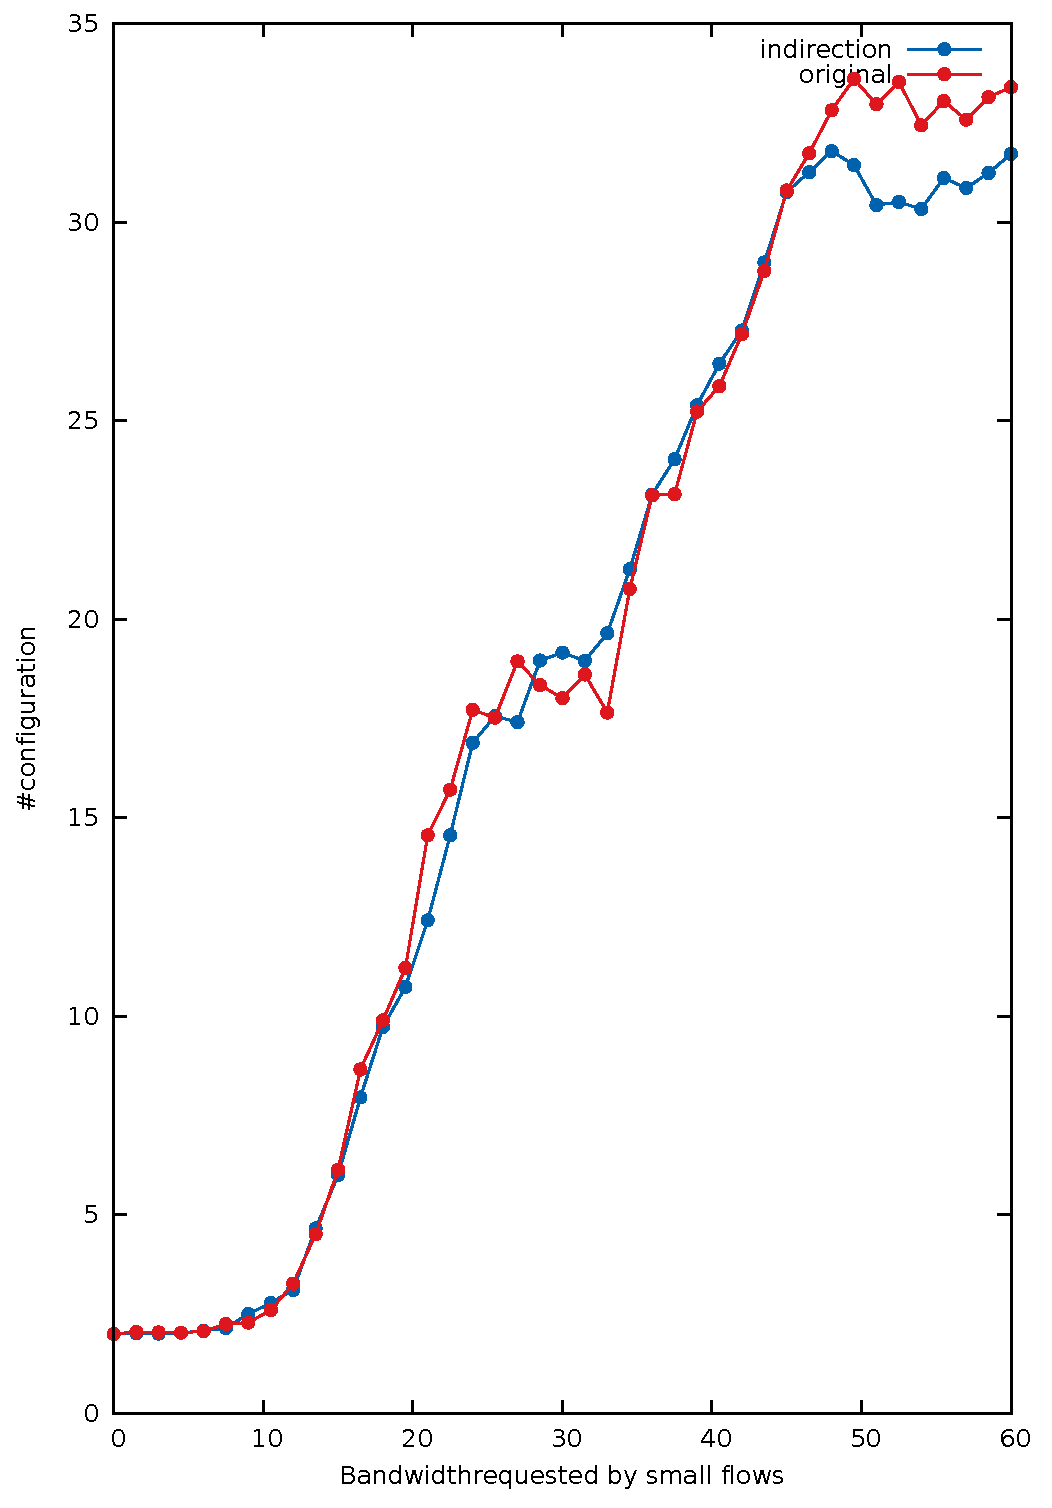
\includegraphics[width=3in]{figures/ndayRandom}
		\caption{Configuration number with random selection}
		\label{fig:ndayRandom}
	\end{minipage}%
	\qquad
	\begin{minipage}{3in}%
		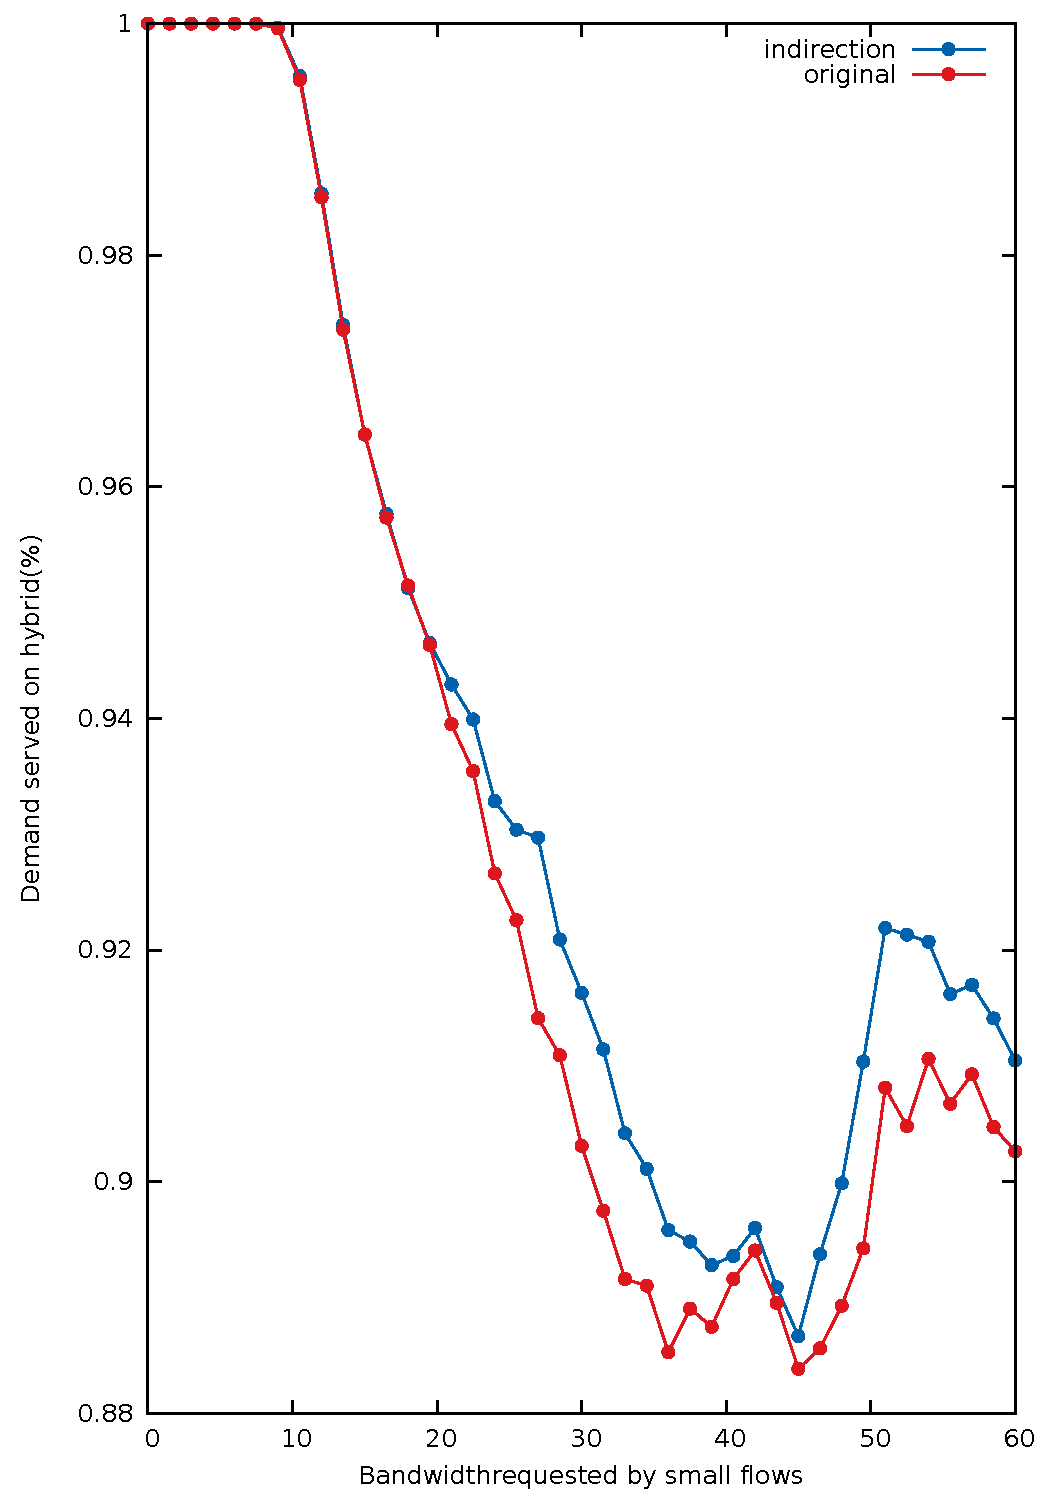
\includegraphics[width=3in]{figures/ndem3Random}
		\caption{Demand served by hybrid switch with random selection}
		\label{fig:ndem3Random}
	\end{minipage}%
\end{figure}

Figure~\ref{fig:ndayRandom} and Figure~\ref{fig:ndem3Random} are experiment result comparison on number of configuration and demand served by hybrid switch. Here we use the random target selection to pick indirection targets in the same row. The x axis of the two figures represents the percentage of demand in small demands. For example, x=30 means 30\% of the whole demand comes from small demands.

From the experiment results we can see that when more demands come from small demands, indirection algorithm can effectively reduce configuration times. When x > 45, the reduction is about 3 configuration times. As a result, more demand can be served on hybrid switch because less time is used on configuration and more time can be used to serve demands. This experiments shows that with simple heuristics, indirection can effectively improve the hybrid switch performance. When x is bigger than 45, 1 - 2 percent more demand can be served on hybrid switch using indirection. The absolute increase is not significant but if we consider that 90\% of the demand has already been served by hybrid switch by using Solstice algorithm, the relative improvement is reasonable.

\begin{figure}
	\centering
	\begin{minipage}{3in}%
		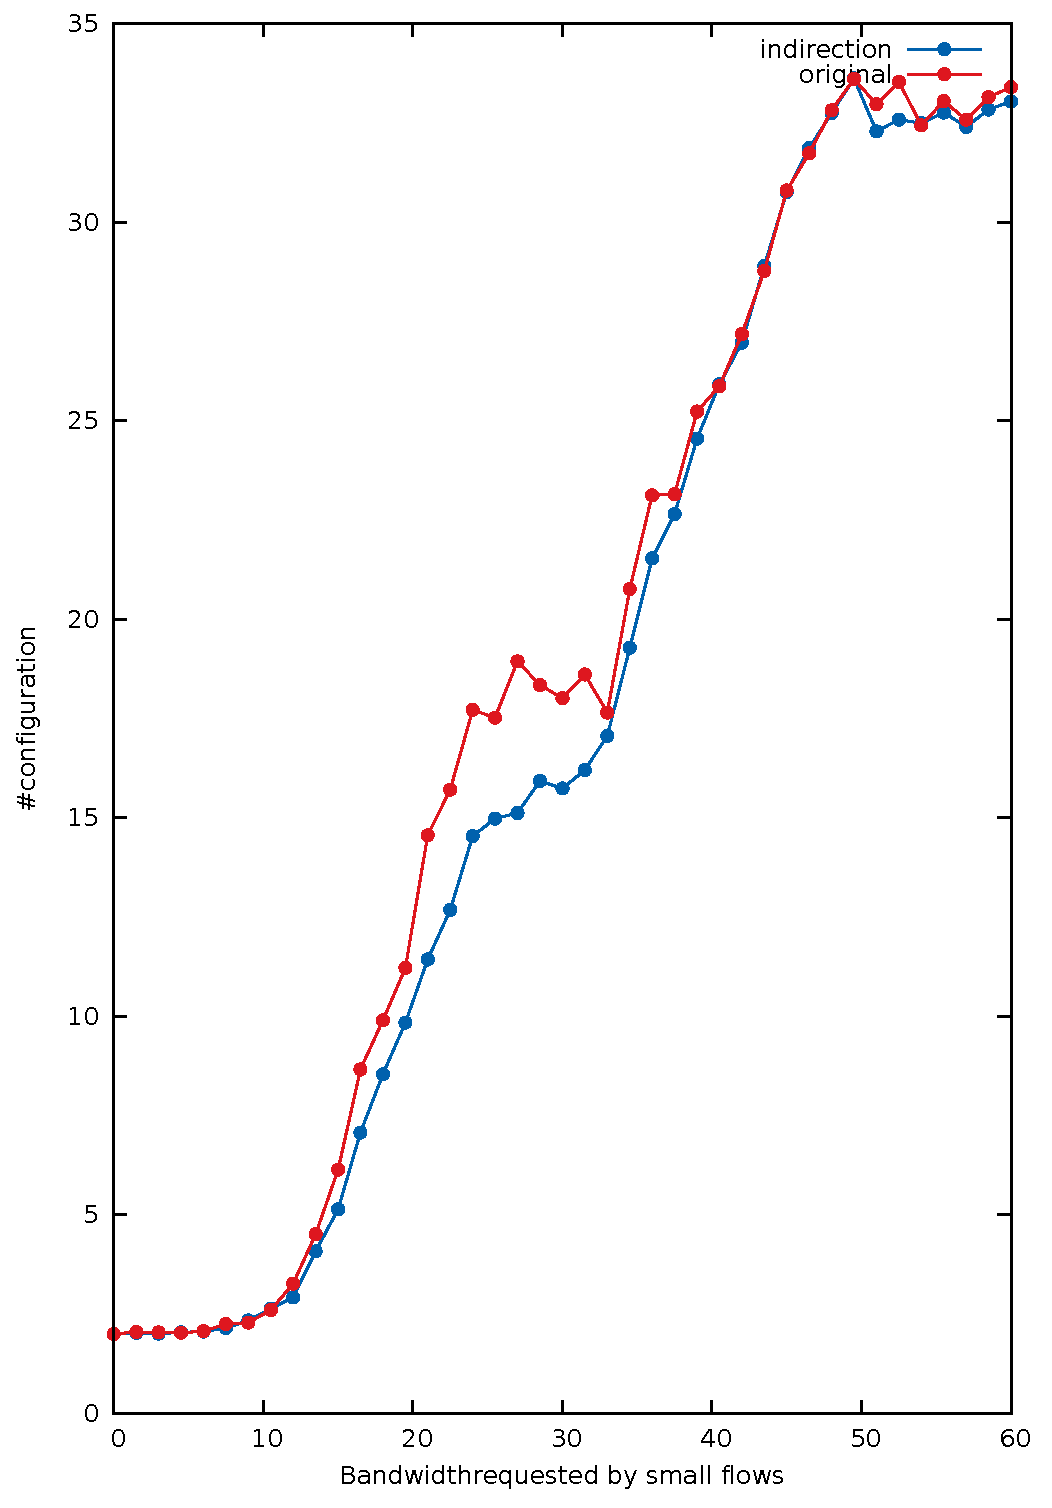
\includegraphics[width=3in]{figures/ndaySorted}
		\caption{Configuration number with largest entry first selection}
		\label{fig:ndaySorted}
	\end{minipage}%
	\qquad
	\begin{minipage}{3in}%
		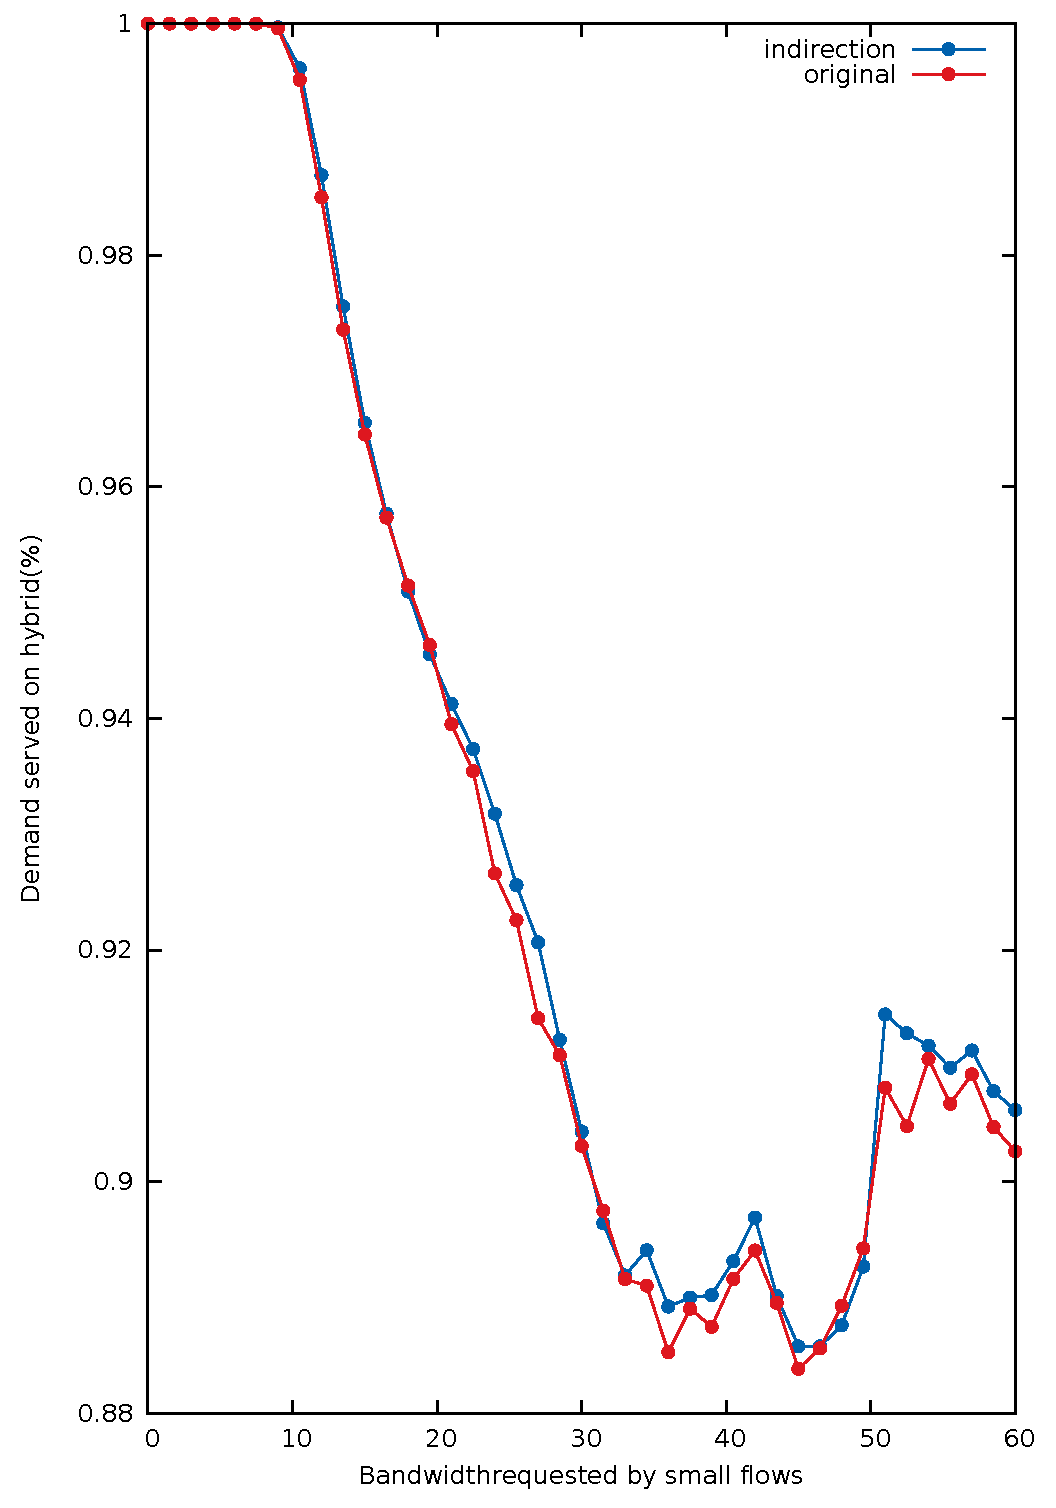
\includegraphics[width=3in]{figures/ndem3Sorted}
		\caption{Demand served by hybrid switch with largest entry first selection}
		\label{fig:ndem3Sorted}
	\end{minipage}%
\end{figure}

Figure~\ref{fig:ndaySorted} and Figure~\ref{fig:ndem3Sorted} are experiment result comparison with Solstice and indirection with largest entry first selection. We just change the selection strategy in the scheduling algorithm but the figure shape differs a lot from the previous experiment. When x is very large (e.g. x > 45), indirection does not see great advantages to the Solstice scheduling algorithm. But in the previous experiments with random selection, we do see improvements there. The improvements of using largest entry first in in the middle part. That is because large entries are filled up when about 30\% of demand come from small demands. Then few demand can be indirected to large entries. 


\section{Conclusion}
\label{sec:conclusion}
In this paper, we investigated the use of indirection in hybrid switch scheduling problem. We formulated the scheduling problem into an integer linear programming problem and solved the problem with and without the use of indirecton. The optimal solution given by ILP shows that indirection can successfully reduce configuration times and increase the demand served by hybrid swithch in a skewed traffic pattern. The ILP optimal solution shows the potential benefits of using the indirection scheduling algorithm. To prove the practical benefit of indirection, we designed and implemented an indirection scheduling algorithm based on simple heuristics. Experiment results show that even an algorithm based on very simple heuristics can achievie reasonable improvements over the direct-path algorithm. 


%\appendix
%\input{appendix_sources}

%\vspace{-0.1in}
%\section*{Acknowledgments}
% Comments for people we need to ack in the final version

\bibliography{ref}
\bibliographystyle{abbrvnat}

\end{document}

% Local Variables:
% TeX-command-default: "LaTeX PDF"
% End:

